\documentclass[a4paper,11pt,oneside]{article}

\usepackage{amsmath,amssymb,epsfig}
\usepackage{url}
\usepackage[T1]{fontenc}
\usepackage{ae,aecompl}
\usepackage{subfigure}
\addtolength{\voffset}{-1cm}
\addtolength{\hoffset}{-1cm}
\setlength{\parindent}{0in}
\addtolength{\textwidth}{1.8cm}
\addtolength{\textheight}{1cm}
\addtolength{\parskip}{.5cm}
% Example definitions.
% --------------------
\def\e{{e^{j\omega}}}
\def\W{{W_M}}
\def\sumk{{\sum_{k=-\infty}^{\infty}}}
\def\x{{\mathbf x}}
\def\X{{\mathbf X}}
\def\u{{\mathbf u}}
\def\U{{\mathbf U}}
\def\x{{\mathbf x}}
\def\s{{\mathbf s}}
\def\A{{\mathbf A}}
\def\y{{\mathbf y}}
\def\w{{\mathbf w}}
\def\B{{\mathbf B}}
\def\a{{\mathbf a}}
\def\D{{\mathbf D}}
\def\P{{\mathbf P}}
\def\n{{\mathbf n}}
\def\V{{\mathbf V}}
\def\R{{\mathbf R}}
\def\I{{\mathbf I}}
\def\M{{\mathbf M}}
\def\sech{{\mathrm{sech}}}
\def\L{{\cal L}}
\def\Cum{{\rm{Cum}}}
\def\var{{\rm{var}}}
\def\T{{\mathbf T}}
\def\C{{\mathbf C}}
\def\tf{{\emph{t-f}}}

% Title.
% ------
\title{\large{\textbf{EXERCISE 3}}}
\author{SGN-1156 Signal Processing Techniques\\
\texttt{http://www.cs.tut.fi/courses/SGN-1156}\\
Tampere University of Technology\\
Germ\'an G\'omez-Herrero, \url{http://germangh.com}}

\date{November 17, 2009}


\begin{document}
\maketitle

\textbf{QUESTION:} Shown in Fig.~\ref{fig1} are two different ways of cascading an up-sampler with a down-sampler. Find and prove the conditions under which the two systems are identical. 



\begin{figure}[h!]
\centering
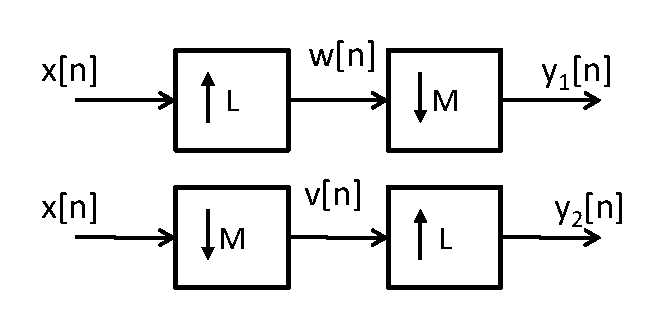
\includegraphics[width=.5\textwidth]{fig3.eps}
\caption{Two ways of cascading and up-sampler and a down-sampler.}
\label{fig1}
\end{figure}

\vspace{1cm}

There are two ways of prove the conditions under which the two systems are identical. The first way does it in the time domain and the second one does it in the Fourier domain. 

\textbf{SOLUTION 1 (time-domain):}

The output of an upsampler in time domain is given by:

\[
w[n] = \left\{
\begin{array}{lll}
x[\frac{n}{L}] & \quad& \textrm{if}\; \frac{n}{L} \in \mathbb{Z}\\
0 &\quad& \textrm{otherwise}
\end{array}
\right.
\]

After downsampling $w[n]$ by an integer factor $M$ we obtain that:

\[
y_1[n]=x[nM]=\left\{
\begin{array}{lll}
x[\frac{nM}{L}] & \quad& \textrm{if}\; \frac{nM}{L} \in \mathbb{Z}\\
0 &\quad& \textrm{otherwise}
\end{array}
\right.
\]

In the second system, we have that:

\[
v[n] = x[nM]
\]

and that the output of the upsampler block is:

\[
y_2[n] = \left\{
\begin{array}{lll}
v[\frac{n}{L}] & \quad& \textrm{if}\; \frac{n}{L} \in \mathbb{Z}\\
0 &\quad& \textrm{otherwise}
\end{array}
\right.
\]

which means that the relationship between $y_2[n]$ and $x[n]$ is:

\[
y_2[n]=\left\{
\begin{array}{lll}
x[\frac{nM}{L}] & \quad& \textrm{if}\; \frac{n}{L} \in \mathbb{Z}\\
0 &\quad& \textrm{otherwise}
\end{array}
\right.
\]


Intuitively, one can see that if $M$ and $L$ has any common factor greater than 1 then $\frac{nM}{L}=\frac{nJ}{K}$ where $\frac{J}{K}$ is in lowest terms and therefore:

\[
\frac{nM}{L}=\frac{nJ}{K}\in\mathbb{Z} \qquad \forall \; n\in A=\left\{0,\pm K,\pm 2K,\pm 3K...\right\}
\]

whereas:

\[
\frac{n}{L}\in\mathbb{Z} \qquad \forall \; n\in B=\left\{0,\pm L,\pm 2L,\pm 3L...\right\}
\]


For $y_1[n]$ to be equal to $y_2[n]$ the series $A$ and $B$ must contain the same elements in the same order, which is not true because, if $M$ and $L$ have any common factor greater than 1 we will have that $K<L$ and therefore the series $A$ contains elements that are not in the series $B$. So this proves that:

\[
\textrm{M and L are NOT relatively prime} \Rightarrow y_1[n]\neq y_{2}[n]
\]

which, by transposition, is equivalent to:

\[
y_1[n]=y_2[n] \Rightarrow \textrm{M and N are relatively prime}
\]

So the condition that $M$ and $N$ are relatively prime is \emph{necessary} for $y_1[n]$ to be equal to $y_1[n]$. However, for the proof to be complete we also have to show that $M$ and $N$ being relatively prime is a \emph{sufficient} condition for $y_1[n]=y_2[n]$, i.e. we have to prove that:

\[
\textrm{M and L are relatively prime}  \Rightarrow  y_1[n]=y_2[n]
\]

Proving the condition above is equivalent to proving:

\[
y_1[n]\neq y_2[n] \Rightarrow \textrm{M and L are not relatively prime}
\]

If $y_1[n]\neq y_2[n]$ this means that the series $A$ and $B$ are not identical, which requires that $K\neq L$ and therefore $\frac{M}{L}$ is not in lowest terms, which means that $M$ and $L$ have a common factor greater than 1, i.e they are not relatively prime. This ends the proof that:

\[
\textrm{M and N are relatively prime}  \Leftrightarrow  y_1[n]=y_2[n]
\]





\textbf{SOLUTION 2 (Fourier domain):}



From Fig.~\ref{fig1} we obtain the following relationships in the DTFT domain:

\[
\left.
\begin{array}{lll}
W(\e) &=& X(e^{j\omega L})\\
Y_1(\e)&=&\frac{1}{M}\sumk W\left(e^{j(\frac{\omega}{M}-\frac{2\pi k}{M})}\right)\\
\end{array}
\right\}
\Rightarrow
Y_1(\e)=\frac{1}{M}\sumk X\left(e^{j(\frac{\omega L}{M}-\frac{2\pi k}{M})}\right)
\]


\[
\left.
\begin{array}{lll}
V(\e) &=& \frac{1}{M}\sumk X\left(e^{j(\frac{\omega}{M}-\frac{2\pi k}{M})}\right)\\
Y_2(\e)&=&V(e^{j\omega L})\\
\end{array}
\right\}
\Rightarrow
Y_2(\e)=\frac{1}{M}\sumk X\left(e^{j(\frac{\omega L}{M}-\frac{2\pi k L}{M})}\right)
\]

Therefore, for the two systems to be equivalent we need that $y_1[n]=y_2[n]\Rightarrow Y_1(\e)=Y_2(\e)$, which means that we need to find the relationship between $M$ and $L$ so that the following equality holds:

\begin{equation}\label{eq1}
\sumk X\left(e^{j(\frac{\omega L}{M}-\frac{2\pi k}{M})}\right) = \sumk X\left(e^{j(\frac{\omega L}{M}-\frac{2\pi k L}{M})}\right)
\end{equation}

For notational convenience, we are going to denote in the following $W_M=e^{-j\frac{2\pi}{M}}$. Then we can write Eq.~\ref{eq1} as:


\begin{equation}\label{eq2}
\sumk X\left(e^{j\frac{\omega L}{M}} W_{M}^{k}\right) = \sumk X\left(e^{j\frac{\omega L}{M}}W_{M}^{kL}\right)
\end{equation}

and then by denoting $A_{k}=W_{M}^k$ and $B_{k}=W_{M}^{kL}$ we can define the following infinite series:

\[
\begin{array}{lll}
\left\{A_{k}\right\}_{k=-\infty}^{\infty}&=&\left\{\overbrace{W_{M}^{-\infty}}^{A_{-\infty}},...,\overbrace{W_{M}^{0}}^{A_{0}},\overbrace{W_{M}^1}^{A_1},...,\overbrace{W_{M}^{M-1}}^{A_{M-1}},\overbrace{W_{M}^{M}}^{A_M},\overbrace{W_{M}^{M+1}}^{A_{M+1}},...,\overbrace{W_{M}^{\infty}}^{A_{\infty}}\right\}\\
&&\\
\left\{B_{k}\right\}_{k=-\infty}^{\infty}&=&\left\{\underbrace{W_{M}^{-\infty}}_{B_{-\infty}},...,\underbrace{W_{M}^{0}}_{B_0},\underbrace{W_{M}^L}_{B_L},...,\underbrace{W_{M}^{(M-1)L}}_{B_{(M-1)L}},\underbrace{W_{M}^{ML}}_{B_{ML}},\underbrace{W_{M}^{(M+1)L}}_{B_{(M+1)L}},...,\underbrace{W_{M}^{\infty}}_{B_\infty}\right\}
\end{array}
\]


So it is obvious that Eq.~\ref{eq2} takes the form:

\[
\begin{array}{lll}
&&X\left(e^{\frac{\omega L}{M}}A_{-\infty} \right)+...+X\left(e^{\frac{\omega L}{M}}A_{0} \right)+X\left(e^{\frac{\omega L}{M}}A_{1} \right)+...+X\left(e^{\frac{\omega L}{M}}A_{\infty}\right)=\\
&=&X\left(e^{\frac{\omega L}{M}}B_{-\infty} \right)+...+X\left(e^{\frac{\omega L}{M}}B_{0} \right)+X\left(e^{\frac{\omega L}{M}}B_{1} \right)+...+X\left(e^{\frac{\omega L}{M}}B_{\infty}\right)
\end{array}
\]

Indeed, the order of the operands in the summatories above is irrelevant and therefore, for the equality to hold, the series $\left\{A_{k}\right\}$ must contain the same elements as the series $\left\{B_{k}\right\}$, but not necessarily in the same order. If the series $\left\{B_{k}\right\}$ is a re-ordered version of $\left\{A_{k}\right\}$ the equality still holds.

Moreover, note that for any two integers $k$ and $r$ we have that:

 \[
 W_{M}^{k+r M}=W_{M}^{k}W_{M}^{r M}=W_{M}^{k}e^{j2\pi r}=W_{M}^{k}
 \]

This means that for any integer $r$ we have that $A_{k+rM}=W_{M}^{k+rM}=W_{M}^{k}=A_{k}$ and that $B_{k+rM}=W_{M}^{k+rM}=W_{M}^{k}=B_{k}$. So both the series $\left\{A_{k}\right\}$ and $\left\{B_{k}\right\}$ are periodic with a period equal to $M$, i.e.:

\[
\begin{array}{lll}
\left\{A_{k}\right\}_{k=-\infty}^{\infty} &=& \left\{...,\overbrace{A_0,A_1,...,A_{M-1}}^{\textrm{1 period of length M}},A_0,A_1,...,A_{M-1},...\right\}\\
&&\\
\left\{B_{k}\right\}_{k=-\infty}^{\infty} &=& \left\{...,\underbrace{B_0,B_1,...,B_{M-1}}_{\textrm{1 period of length M}},B_0,B_1,...,B_{M-1},...\right\}\\
\end{array}
\]

So saying that the infinite series $\left\{B_{k}\right\}_{k=-\infty}^{\infty}$ must contain the same elements (possibly re-ordered) as the infinite series $\left\{A_{k}\right\}_{k=-\infty}^{\infty}$ is the same as saying that the finite series $\left\{B_{k}\right\}_{k=0}^{M-1}$ contains the same elements (possibly reordered) as the finite series $\left\{A_{k}\right\}_{k=0}^{M-1}$.

Recall that any complex exponential $C \cdot e^{j\theta}$ where $C$ is a positive constant can be represented in an \emph{Argand diagram} as a vector of length $C$ that forms an angle $\theta$ with the horizontal axis. An Argand diagram can be understood as a cartesian diagram in which the vertical axis represents the imaginary part of a given complex number and the horizontal axis represents the real part. See Fig.~\ref{arganddiagram} for an example of an Argand diagram.


\begin{figure}[h!]
\centering
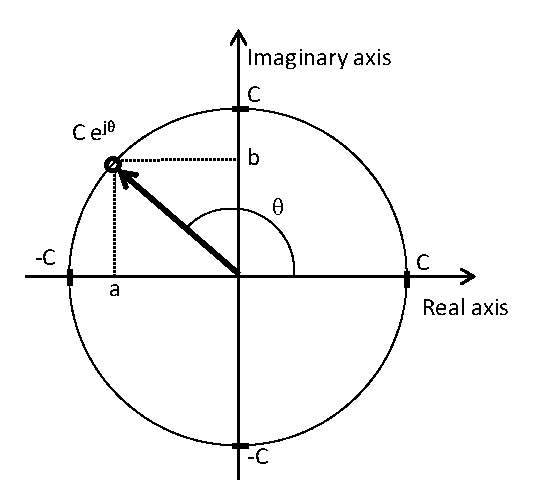
\includegraphics[width=.6\textwidth]{arganddiagram.eps}
\caption{Vectorial representation of a complex exponential $Ce^{j\theta}=C(\cos \theta + j\sin \theta)=a+jb$ using an Argand diagram. The length of the depicted vector is equal to $C$.}
\label{arganddiagram}
\end{figure}


Using an Argand diagram we can represent the elements in the series  $\left\{A_{k}\right\}_{k=0}^{M-1}$ as is shown in Fig.~\ref{argandA} from where we can see that the $M$ elements of that series are different from each other. In Fig.~\ref{argandB} we plot the possible values that each element of the series $\left\{B_{k}\right\}_{k=0}^{M-1}$ can take. From those figures it becomes clear that each element of the series $\left\{B_{k}\right\}_{k=0}^{M-1}$, say $B_{n}$, can only take one of the $M$ different values $\{A_0,A_1,...,A_{M-1}\}$. Then we can conlude that $\left\{B_{k}\right\}_{k=0}^{M-1}$ will be just a re-ordered version of $\left\{A_{k}\right\}_{k=0}^{M-1}$ whenever $\left\{B_{k}\right\}_{k=0}^{M-1}$ does not contain any repeated values. For this to happen we must have that for any two different integers $0<\alpha<M-1$ and $0<\beta<M-1$ the angles $\alpha\theta$ and $\beta\theta$ are different ($\theta$ is the angle showed in Fig.~\ref{argandA} and Fig.~\ref{argandB}). For this to happen we must have that, for an integer $r$:

\[
\alpha L\theta \neq \beta L\theta + rM\theta \Rightarrow (\alpha-\beta)L \neq rM \Rightarrow \gamma L \neq rM 
\]

where $r$ is any integer and $\gamma$ is an integer in the range $1\leq \gamma \leq M-1$. This means that $L$ and $M$ cannot have any common divisor greater than 1. So the two systems are identical if and only if $M$ and $L$ are relatively prime.


\begin{figure}[h!]
\centering
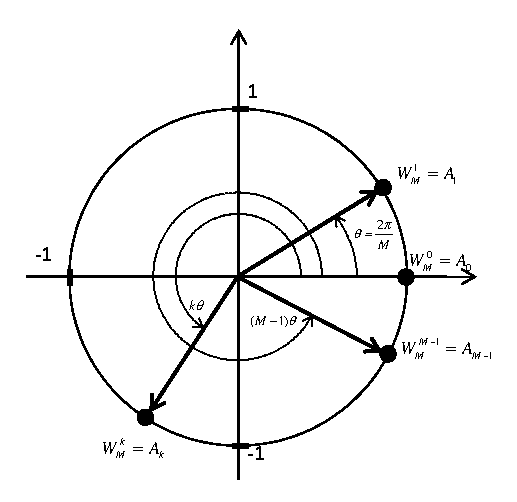
\includegraphics[width=.6\textwidth]{argandA.eps}
\caption{Vectorial representation of the elements of the series $\left\{A_{k}\right\}_{k=0}^{M-1}$. Note that the vector representing element $A_{n}$ is obtained by rotating $A_{n-1}$ an angle $\theta=\frac{2\pi}{M}$. Note also how the element $A_{0}$ is obtained by rotating $A_{M-1}$ by an angle $\theta$. Obviously, each of these $M$ vectors is \emph{different} from each other which means that all the elements of the series $\left\{A_{k}\right\}_{k=0}^{M-1}$ are different from each other.}
\label{argandA}
\end{figure}




\begin{figure}[h!]
\centering
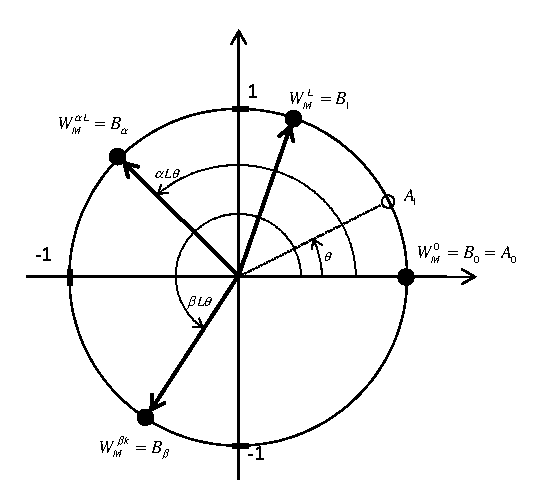
\includegraphics[width=.6\textwidth]{argandB.eps}
\caption{Vectorial representation of the elements of the series $\left\{B_{k}\right\}_{k=0}^{M-1}$. Note that the vector representing element $B_{n}$ is obtained by rotating $B_{n-1}$ an angle $L\theta=\frac{2\pi L}{M}$. Note also that both $\left\{B_{k}\right\}_{k=0}^{M-1}$ and $\left\{A_{k}\right\}_{k=0}^{M-1}$ have the same starting point, i.e. $B_0=A_0$. Because the elements of $\left\{B_{k}\right\}_{k=0}^{M-1}$ are obtained by rotating $B_{0}$ an angle equal to an integer multiple of $\theta$ it is obvious that an arbitrary element, say $B_{k}$ can only take one of the values $\{A_{0},A_1,...,A_{M-1}\}$.}
\label{argandB}
\end{figure}




\end{document}